\section{Analyse}

In diesem Kapitel wird die bestehende Situation im Budget-Controlling analysiert und die Anforderungen an die zu entwickelnde Middleware definiert. Die Analyse folgt nach \cite{sommerville2015} einem strukturierten Vorgehen: Zunächst wird der Ist-Zustand erfasst, anschließend werden funktionale und nicht-funktionale Anforderungen abgeleitet.

\subsection{Ist-Analyse}

\subsubsection{Excel-basierter Workflow}

Der aktuelle Workflow basiert auf einer zentralen Excel-Datei (\texttt{Budgetcontrolling.xlsx}), welche über SharePoint geteilt wird. Die Datei integriert Daten aus verschiedenen Quellen mittels Power Query.

\begin{table}[H]
\centering
\caption{Sheets in Budgetcontrolling.xlsx}
\label{tab:excel-sheets}
\begin{tabularx}{\textwidth}{l>{\raggedright\arraybackslash}Xl}
\toprule
\textbf{Sheet} & \textbf{Zweck} & \textbf{Quelle} \\
\midrule
qry\_CALM\_Data & User Stories mit \gls{psp}-Zuordnung & Power Query \\
CADO & Zeitbuchungen (Ist-Stunden) & SAP-Export \\
PSP-Elemente & Budget pro \gls{psp} & Manuell \\
1. PSP-Zuordnung & Manuelle Zuordnungen & Manuell \\
2. PSP-Zuordnung & Fallback: Team $\rightarrow$ Timebox $\rightarrow$ \gls{psp} & Manuell \\
Reporting & Zusammenfassung pro Team & Berechnet \\
\bottomrule
\end{tabularx}
\end{table}

\subsubsection{Budget-Metriken}

Die folgenden Metriken werden für das Budget-Controlling verwendet. Diese Kennzahlen entsprechen den im Projektmanagement etablierten Earned Value Management (EVM) Metriken \citep{kerzner2017, pmi2021}:

\begin{table}[H]
\centering
\caption{Budget-Metriken und ihre Berechnung}
\label{tab:metriken}
\begin{tabularx}{\textwidth}{l>{\raggedright\arraybackslash}Xl}
\toprule
\textbf{Metrik} & \textbf{Beschreibung} & \textbf{Berechnung} \\
\midrule
Budget & Geplantes Budget & Summe aus PSP-Elemente \\
Actual & Bereits geleistete Arbeit & CADO Stunden / 8 \\
\gls{etc} & Noch zu leistende Arbeit & qry\_CALM\_Data (mit \gls{psp}) \\
\gls{eac} & Geschätzte Gesamtkosten & Actual + \gls{etc} \\
\bottomrule
\end{tabularx}
\end{table}

Zur Veranschaulichung ein Beispiel: Für ein Team mit einem geplanten Budget von 120~PT wurden bisher 55,53~PT tatsächlich geleistet (Actual), die aus den CADO-Zeitbuchungen berechnet werden (444,24 Stunden / 8). Der verbleibende Restaufwand (ETC) beträgt laut den User Stories mit \gls{psp}-Zuordnung 63,88~PT. Daraus ergibt sich eine Gesamtprognose (EAC) von 119,41~PT (55,53 + 63,88), die in diesem Fall knapp unter dem Budget liegt.

\subsubsection{Problemanalyse}

Die Analyse des bestehenden Workflows offenbart mehrere Probleme. Zunächst stehen keine Echtzeitdaten zur Verfügung, da Power Query nur bei manuellem Refresh aktualisiert wird. Darüber hinaus existiert keine API, über die andere Systeme auf die Daten zugreifen könnten. \gls{psp}-Zuordnungen müssen manuell in Excel gepflegt werden, wobei keine automatische Prüfung auf Konsistenz stattfindet. Schließlich werden Änderungen nicht nachvollziehbar protokolliert, sodass eine Historisierung fehlt.

\subsection{Soll-Konzept}

Die Middleware soll die beschriebenen Probleme lösen und gleichzeitig einen einfachen Übergang zu einer service-orientierten Architektur ermöglichen. Middleware bezeichnet dabei Software, die als Vermittlungsschicht zwischen verteilten Anwendungen fungiert und deren Kommunikation vereinfacht \citep{bernstein1996, tanenbaum2017}. Das Konzept folgt dem Prinzip der \enquote{Strangler Fig Application}, bei dem eine neue Architektur schrittweise die alte ersetzt \citep{newman2021}.

\begin{figure}[H]
\centering
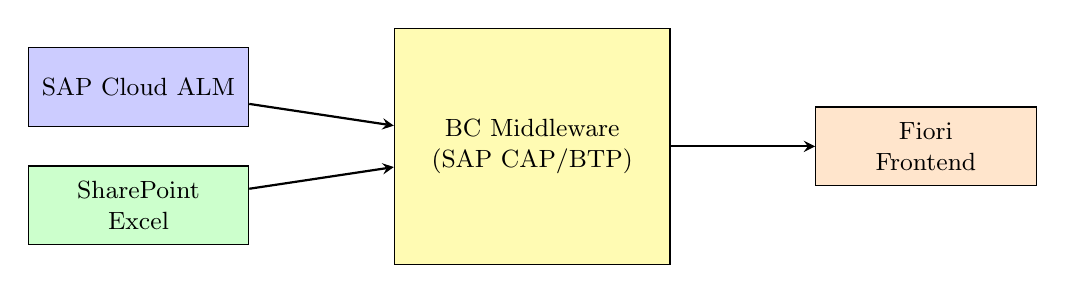
\begin{tikzpicture}[
    box/.style={rectangle, draw, minimum width=2.8cm, minimum height=1cm, align=center, font=\small},
    arrow/.style={->, >=stealth, thick}
]
    % Datenquellen links
    \node[box, fill=blue!20] (calm) at (0,1.5) {SAP Cloud ALM};
    \node[box, fill=green!20] (sharepoint) at (0,0) {SharePoint\\Excel};

    % Middleware Mitte
    \node[box, fill=yellow!30, minimum width=3.5cm, minimum height=3cm] (middleware) at (5,0.75) {BC Middleware\\(SAP CAP/BTP)};

    % Frontend rechts
    \node[box, fill=orange!20] (frontend) at (10,0.75) {Fiori\\Frontend};

    % Pfeile
    \draw[arrow] (calm) -- (middleware);
    \draw[arrow] (sharepoint) -- (middleware);
    \draw[arrow] (middleware) -- (frontend);
\end{tikzpicture}
\caption{Soll-Architektur der BC Middleware}
\label{fig:soll-architektur}
\end{figure}

Abbildung~\ref{fig:soll-architektur} zeigt die Zielarchitektur. Die zentrale Idee besteht in der Entkopplung des Frontends von der konkreten Datenquelle. Das Frontend kommuniziert ausschließlich mit der Middleware über eine standardisierte \gls{odata}-Schnittstelle. Die Middleware abstrahiert die Komplexität des Datenzugriffs und ermöglicht einen transparenten Wechsel zwischen Excel- und Service-Backend.

\subsection{Verwandte Arbeiten}

Die Problemstellung der vorliegenden Arbeit berührt mehrere Forschungsbereiche, die im Folgenden eingeordnet werden.

\subsubsection{Middleware und Integrationsarchitekturen}

Das Konzept der Middleware als Vermittlungsschicht zwischen heterogenen Systemen ist seit den 1990er Jahren etabliert \citep{bernstein1996}. \cite{emmerich2000} identifizierte Middleware als zentrales Element für die Integration verteilter Systeme und prognostizierte deren wachsende Bedeutung. Die Enterprise Integration Patterns von \cite{hohpe2003} bieten einen umfassenden Katalog von Integrationsmustern, darunter das in dieser Arbeit verwendete Adapter-Pattern.

\subsubsection{Spreadsheet-basierte Systeme in Unternehmen}

Die Verbreitung und Risiken von Spreadsheet-Anwendungen in Unternehmen sind Gegenstand umfangreicher Forschung. \cite{panko2016} beschreiben Tabellenkalkulationen als \enquote{Dark Matter} der Unternehmens-IT -- allgegenwärtig, aber schwer zu kontrollieren. \cite{powell2009} dokumentieren in ihrer Metastudie, dass Spreadsheets häufig Fehler enthalten und dennoch für geschäftskritische Entscheidungen verwendet werden. Diese Erkenntnisse unterstreichen die Relevanz von Lösungen, die einen kontrollierten Übergang zu strukturierteren Systemen ermöglichen.

\subsubsection{Abgrenzung}

Im Unterschied zu bestehenden Arbeiten, die sich primär auf die Fehleranalyse von Spreadsheets oder allgemeine Integrationsarchitekturen konzentrieren, adressiert diese Arbeit die spezifische Fragestellung der Backend-Austauschbarkeit im SAP-Kontext. Der Fokus liegt auf der praktischen Umsetzung einer Architektur, die sowohl Excel-basierte als auch service-orientierte Backends unterstützt.

\subsection{Stakeholder-Analyse}

Für den erfolgreichen Entwurf der Middleware ist das Verständnis der beteiligten Stakeholder und ihrer Anforderungen essentiell \citep{sommerville2015}.

\begin{table}[H]
\centering
\caption{Stakeholder und ihre Interessen}
\label{tab:stakeholder}
\begin{tabularx}{\textwidth}{l>{\raggedright\arraybackslash}X>{\raggedright\arraybackslash}X}
\toprule
\textbf{Stakeholder} & \textbf{Rolle} & \textbf{Interesse} \\
\midrule
Projektleiter & Nutzt Budget-Reports für Entscheidungen & Aktuelle, korrekte Zahlen; einfache Bedienung \\
\midrule
Controller & Pflegt Budgetdaten und PSP-Zuordnungen & Effiziente Dateneingabe; Konsistenzprüfung \\
\midrule
Frontend-Entwickler & Entwickelt Fiori-Oberfläche & Stabile, dokumentierte API; OData-Konformität \\
\midrule
IT-Architekten & Plant zukünftige Integration & Austauschbarkeit; saubere Architektur \\
\midrule
SAP-Administratoren & Betreibt die Anwendung auf BTP & Einfaches Deployment; Monitoring \\
\bottomrule
\end{tabularx}
\end{table}

\subsection{Use Cases}

Die folgenden Use Cases beschreiben die wichtigsten Interaktionen mit dem System. Use Cases sind ein bewährtes Mittel der Anforderungsanalyse, um funktionale Anforderungen aus Nutzersicht zu dokumentieren \citep{sommerville2015}:

\subsubsection{UC-01: Budget-Übersicht abrufen}

\begin{table}[H]
\centering
\begin{tabularx}{\textwidth}{l>{\raggedright\arraybackslash}X}
\toprule
\textbf{Akteur} & Projektleiter \\
\midrule
\textbf{Vorbedingung} & Benutzer hat Session gestartet \\
\midrule
\textbf{Ablauf} &
1. Benutzer öffnet Budget-Dashboard \\
& 2. Frontend ruft GET /BudgetOverview auf \\
& 3. Middleware lädt Excel, berechnet Metriken \\
& 4. Frontend zeigt Budget/Actual/ETC/EAC pro Team \\
\midrule
\textbf{Nachbedingung} & Aktuelle Budget-Metriken werden angezeigt \\
\bottomrule
\end{tabularx}
\caption{Use Case: Budget-Übersicht abrufen}
\end{table}

\subsubsection{UC-02: PSP-Zuordnung erstellen}

\begin{table}[H]
\centering
\begin{tabularx}{\textwidth}{l>{\raggedright\arraybackslash}X}
\toprule
\textbf{Akteur} & Controller \\
\midrule
\textbf{Vorbedingung} & User Story existiert ohne PSP-Zuordnung \\
\midrule
\textbf{Ablauf} &
1. Controller wählt User Story aus Liste \\
& 2. Controller wählt PSP-Element aus Dropdown \\
& 3. Frontend ruft POST /createPSPAssignment auf \\
& 4. Middleware schreibt Zuordnung in Excel \\
& 5. Bestätigung wird angezeigt \\
\midrule
\textbf{Nachbedingung} & User Story ist PSP zugeordnet; ETC wird berechnet \\
\midrule
\textbf{Alternativ} & Bei Team-Mismatch: Warnung anzeigen \\
\bottomrule
\end{tabularx}
\caption{Use Case: PSP-Zuordnung erstellen}
\end{table}

\subsubsection{UC-03: Projekt wechseln}

\begin{table}[H]
\centering
\begin{tabularx}{\textwidth}{l>{\raggedright\arraybackslash}X}
\toprule
\textbf{Akteur} & Alle Benutzer \\
\midrule
\textbf{Vorbedingung} & Mehrere Projekte sind konfiguriert \\
\midrule
\textbf{Ablauf} &
1. Benutzer ruft GET /getProjects() auf \\
& 2. Liste verfügbarer Projekte wird angezeigt \\
& 3. Benutzer wählt Projekt aus \\
& 4. POST /startSession mit Projektname \\
& 5. Session-ID wird zurückgegeben und gespeichert \\
\midrule
\textbf{Nachbedingung} & Alle folgenden Requests nutzen das gewählte Projekt \\
\bottomrule
\end{tabularx}
\caption{Use Case: Projekt wechseln}
\end{table}

\subsection{Anforderungsanalyse}

\subsubsection{Funktionale Anforderungen}

\begin{table}[H]
\centering
\caption{Funktionale Anforderungen}
\label{tab:fa}
\begin{tabularx}{\textwidth}{l>{\raggedright\arraybackslash}X}
\toprule
\textbf{ID} & \textbf{Anforderung} \\
\midrule
FA-01 & Das System muss Budget-Metriken pro Team berechnen können \\
FA-02 & Das System muss Budget-Metriken pro \gls{psp} berechnen können \\
FA-03 & Das System muss \gls{crud}-Operationen für \gls{psp}-Zuordnungen unterstützen \\
FA-04 & Das System muss Session-basiertes Projekt-Management unterstützen \\
FA-05 & Das System muss Team-Mismatch-Warnungen generieren können \\
FA-06 & Das System muss Excel-Daten von SharePoint lesen können \\
FA-07 & Das System muss Änderungen zurück in Excel schreiben können \\
\bottomrule
\end{tabularx}
\end{table}

\subsubsection{Nicht-funktionale Anforderungen}

\begin{table}[H]
\centering
\caption{Nicht-funktionale Anforderungen}
\label{tab:nfa}
\begin{tabularx}{\textwidth}{l>{\raggedright\arraybackslash}X}
\toprule
\textbf{ID} & \textbf{Anforderung} \\
\midrule
NFA-01 & Die Backend-Implementierung muss austauschbar sein \\
NFA-02 & Die \gls{api} muss \gls{odata} v4-kompatibel sein \\
NFA-03 & Das System muss auf der SAP \gls{btp} deploybar sein \\
NFA-04 & Die \gls{api} muss für ein Fiori-Frontend geeignet sein \\
NFA-05 & Das System muss ohne lokale Datenbankinstanz funktionieren \\
\bottomrule
\end{tabularx}
\end{table}

\subsection{Priorisierung der Anforderungen}

Die Anforderungen werden nach der MoSCoW-Methode priorisiert \citep{sommerville2015}:

\begin{table}[H]
\centering
\caption{Priorisierung der Anforderungen}
\label{tab:priorisierung}
\begin{tabularx}{\textwidth}{cl>{\raggedright\arraybackslash}X}
\toprule
\textbf{Prio} & \textbf{ID} & \textbf{Anforderung} \\
\midrule
\multirow{4}{*}{\textbf{Must}} & FA-01 & Budget-Metriken pro Team \\
& FA-02 & Budget-Metriken pro PSP \\
& FA-06 & Excel-Daten lesen \\
& NFA-02 & OData v4-kompatibel \\
\midrule
\multirow{3}{*}{\textbf{Should}} & FA-03 & CRUD für PSP-Zuordnungen \\
& FA-04 & Session-Management \\
& NFA-01 & Backend austauschbar \\
\midrule
\multirow{2}{*}{\textbf{Could}} & FA-05 & Team-Mismatch-Warnungen \\
& FA-07 & Excel Write-Back \\
\midrule
\textbf{Won't} & -- & Fiori-Frontend (andere Arbeit) \\
\bottomrule
\end{tabularx}
\end{table}

\subsection{Abgrenzung}

Mehrere Aspekte sind bewusst nicht Bestandteil dieser Arbeit. Das Fiori-Frontend wird von anderen Studierenden im Rahmen separater Arbeiten entwickelt; die vorliegende Arbeit stellt lediglich die API bereit. Die vollständige CALM-Integration wird nur konzeptionell beschrieben, aber nicht implementiert, was dennoch eine Bewertung der Austauschbarkeit ermöglicht. Die Benutzer-Authentifizierung wird durch die SAP BTP (XSUAA Service) bereitgestellt und ist somit nicht Teil der Middleware-Implementierung. Eine vollständige Audit-Trail-Funktionalität für die Historisierung von Änderungen ist ebenso wenig vorgesehen wie eine vollständige Mandantentrennung mit separaten Datenbeständen -- die Middleware unterstützt zwar mehrere Projekte, jedoch keine echte Mandantenfähigkeit.
